
Deep neural networks (DNNs) have achieved strong performance on visual tasks.
The outstanding performance has been demonstrated by training a model with abundant and diverse labeled data
% ,~\eg,
~\cite{deng2009imagenet, lin2014microsoft}.
Despite the importance of data, machine learning researchers have focused mainly on the model and algorithms~\cite{sambasivan2021everyone}.
We should care about the data for training DNNs because unexpected influences can occur by data.
% and there is a lack of data debugging tools.
% We should first curate the dataset well for training the model because unexpected cascades can occur depending on the curated data~\cite{sambasivan2021everyone}.
% However, such abundant and well-curated labeled data are not available.
% The state-of-the-art DNNs suffer from much lower performance in certain types of classes or groups because of data imbalance.

We commonly encounter data imbalance problems categorized into \emph{class} or \emph{group} imbalance problems.
% The data imbalance problems we commonly encounter are mainly categorized into \emph{class} or \emph{group} imbalance problems.
Class imbalance means different data amounts in the classes.
Suppose that we collect animal images on the internet.
Images of rare animals may be found on search engines less than cats or dogs because of human bias for uploading their photograph~\footnote{For example, the number of search results of Tarsier is about 102 times less than Maltese in Google search engine.}.
Group imbalance, on the other hand, stands for different data amounts in the groups.
We may collect data depending on our environments, including preferences, country, and cultural backgrounds.
Suppose we collect a picture of human hands; then, the skin tones can be biased.
% The curator also may collect data depending on their environments\footnote{The skin tones of hands are imbalance~\cite{grady2022pressurevision}.}, such as preference, country, and cultural backgrounds, which implies the \emph{group imbalance problem}.
If we do not care about these biases, the collected dataset becomes imbalanced in terms of classes~\cite{cui2019class,zhang2023deep}, groups~\cite{whang2021responsible}, or both.
% These biases lead the collected dataset to be imbalanced in terms of classes~\cite{cui2019class,zhang2023deep} and groups~\cite{whang2021responsible}.
With such a dataset and the standard supervised learning algorithms based on empirical risk minimization (ERM) principle~\cite{vapnik1999nature}, the classifier will be trained to 
% will
be biased to majority classes~\cite{geirhos2020shortcut}.
Since these problems yield not only substantial performance degradation but also social or ethical issues with biases, researchers have independently developed various algorithms~\cite{arjovsky2019invariant,bahng2020learning,sagawa2019distributionally,teney2020unshuffling,tartaglione2021end, lee2021learning,LfF,liu2021just, kim2022learning,yao2022improving,hwang2022selecmix,kirichenko2023last,cao2019learning,ren2020balanced,samuel2021distributional, shen2016relay,park2022majority,kim2020m2m,liu2019large,zhang2022correct} to overcome these respective problems.

\begin{figure}[t]
    \centering
    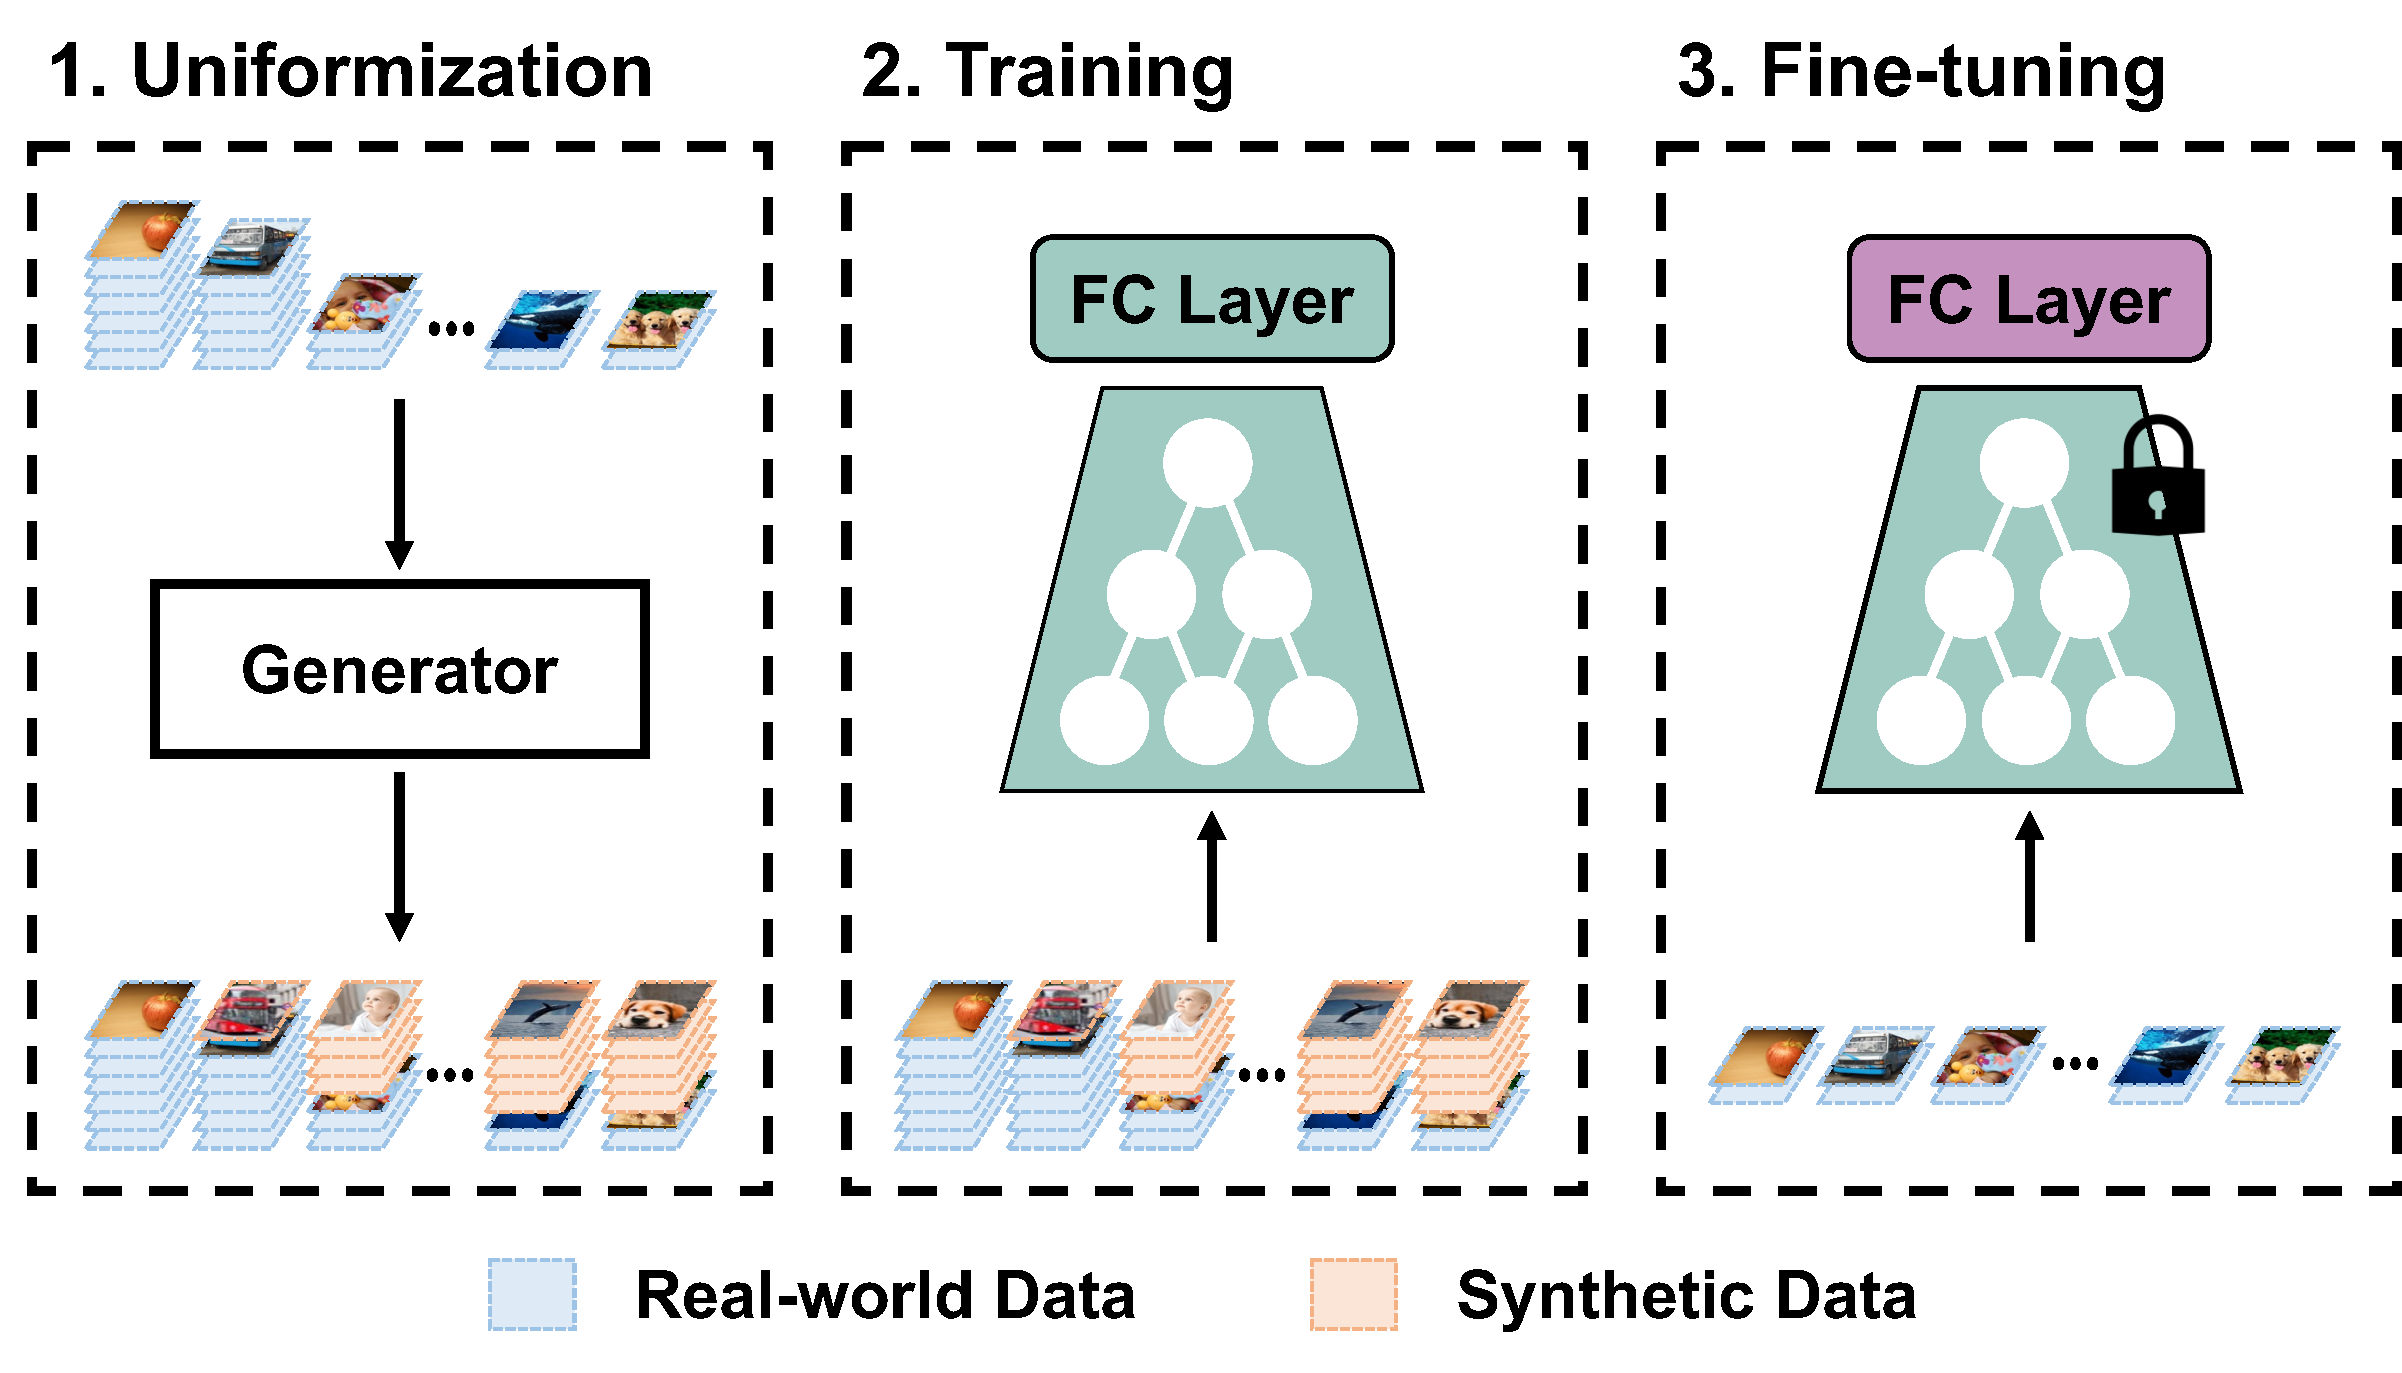
\includegraphics[width=1.0\linewidth]{figures/final.pdf}
    \caption{\textbf{Overview of SYNAuG process.}
    % \textcolor{realblue}{\textbf{legenBlue}} is the real-world data, and \textcolor{synorange}{\textbf{orange}} is the synthetic data.
    Given the imbalanced real-world data with the class labels, we first uniformize the imbalanced real data distribution by generating the synthetic samples that are conditioned on the class label.
    Second, we train a model with the uniformized training data.
    Finally, we fine-tune the last layer with the uniformly subsampled real-world data.}
    \label{fig:overview}
\end{figure}

In this work, we first uniformize the number of samples in each class using the recent text-to-image generative models before applying off-the-shelf task-specific algorithms.
% This takes a different direction, unlike the prior methods.
The prior studies 
% have reported improved performance over the state-of-the-art in their respective tasks.
% However, they use
work the limited, fixed, and bounded original dataset without adding more additional data and mainly focus on algorithmic approaches, such as reweighting~\cite{cao2019learning,ren2020balanced,samuel2021distributional,huang2019deep, ben2009robust, sagawa2019distributionally, jung2023reweighting}, resampling~\cite{shen2016relay,park2022majority,kim2020m2m,liu2019large, kamiran2012data, idrissi2022simple, roh2020fairbatch}, or augmentation~\cite{chuang2021fair, kim2020m2m, park2022majority}.
In contrast to the prior arts, we go beyond the fixed original dataset by exploiting
% , we exploit 
the generative diffusion models to synthesize data, which have recently shown potential as synthetic training data generation~\cite{poole2023dreamfusion, raj2023dreambooth3d, chen2023fantasia3d,trabucco2023effective, he2022synthetic, azizi2023synthetic}.
This allows us to tackle the fundamental bottleneck of data imbalance, \ie, data, rather than indirect ways of tackling learning algorithms or architectures.
It is a more natural way than restricting training data to the fixed dataset as in the prior arts.
% , which would be unnecessary in the generative model era.
% In the generative model era, we argue that restricting training data to the fixed dataset is impractical.
% Furthermore, data imbalance problems should be tackled from the data level before deploying algorithmic approaches.
% so that the practitioners take the controllability of data to mitigate and stabilize the base conditions of datasets.

As shown in \Fref{fig:overview}, we propose SYNAuG, exploiting the generative diffusion model to augment and make the original data distribution to be uniform distribution, \ie, uniformization.
% uniformize the original training data.
% , motivated by recent class imbalance approaches~\cite{kim2020m2m,he2022synthetic,kirichenko2023last}.
After training on the uniformized data composed of the original and synthetic data, we found that it is effective to use simple fine-tuning of the last layer with uniformly sub-sampled original data.
% after pretraining on the mixed dataset.
This outperforms the other strong baselines, including the baseline using the additional external web data as well as the competing methods on the long-tailed recognition benchmark, CIFAR100-LT, and the fairness benchmark, UTKFace.
In addition, we demonstrate the effectiveness of our method for improving the robustness of the classifier to spurious correlation.
We summarize our contributions as follows:
\begin{itemize}
    \item Proposing SYNAuG that uniformizes the given data distribution with synthetic data, beyond the given datasets;\vspace{-1mm}
    % not restricted to the given datasets;
    \item Demonstrating the effectiveness of SYNAuG on three distinctive data imbalance tasks: long-tailed recognition, model fairness, and robustness to spurious correlation;
    \vspace{-1mm}
    \item Reporting the observation of the importance of a few original samples when we use synthetic data together.
\end{itemize}



